\section{Construction and 3D-Print of Design}
The final design differs significantly from the prototypes. It has seen many iterative improvements and thus deserves its' own chapter to cover all the changes to each component of the design. The final design consists of the following bodies:
\begin{enumerate}
	\item{\textbf{Stand}} Is the stand upon which the device resides. Needed for introduction an another axis of rotation and decoupling dispense and disposal mechanisms
	\item{\textbf{UpperBody}} Consists of a walls and a floor of a dispense mechanism with a cutout for dispense and disposal paths as well as connection mechanisms.
	\item{\textbf{UpperMill}} Is a mechanisms that divides the whole dispense system into 21 functional + 1 service chamber (22 in total). Inner side contains a gear and teeth for connecting upper mill with the lower mill (synchronicity between them is still retained)
	\item{\textbf{LowerMill}} Is a mechanisms that divides the whole disposal system into 22 chambers. Unlike dispense system, they are all the same, since chambers need to be of the same size as dispense system, but there is no need for the service chamber. it also contains grooves to reduce the surface contact with lower body and thus friction
	\item{\textbf{LowerBody}} is a very complex detail. Firstly, it contains cutouts for the stepper motor, driver and the deck that holds further electronics. Secondly, it has "ears" that define the axis of rotation for the dispense pathway. Thirdly, it contains grooves for the lower mill to travel on rotationally, to optimize power spent on overcoming friction.
	\item{\textbf{LowerDeck}} Is a cover for all the electronics inside. It contains grooves on the sides for it to slide into electronics chamber.
	\item{\textbf{Electronics}} is the housing for microcontroller, battery and charger. it also contains cutout for the deck to slide into so that electronics is covered from the outside.
	\item{\textbf{Holder}} is a mechanism of additional mechanical fixation of the electronics. Although the Electronics compartment was designed so, that all the components are fixed in place, it might come to the situations where excess movement (e.g. during transportation) might cause electronics to fall out. this mechanism prevents it.
	\item{\textbf{UpperDeck}} Is an upper cover of the device.
\end{enumerate}

Moving forward, we will go step-by-step into the design of each of those components and also will cover the nuances of 3D-printing them all. For now, however, we will compare the final design with the goals set and why this design was chosen in the end. The goals can be divided into 2 types: Initial requirements and the problems arisen during previous designs. Initial requirements are:
\begin{enumerate}
	\item{\textbf{The device contains 21 chambers, 3 for each day of the week.}} This requirement is satisfied. The final design has 22 chambers, 21 of which can contain pills.
	\item{\textbf{The device contains a pill disposal system.}} This requirement is also satisfied. 
	\item{\textbf{The device has an accompanying app for remote control.}} This is not implemented yet. Alternatively, this requirement tells us, that an user interface on the body of device itself is not required. The electronics of this device are chosen so that this requirement can be implemented later on.
\end{enumerate}
The problems that arisen during the design are solved:
\begin{enumerate}
	\item{From first prototype:}
	\begin{enumerate}
		\item{\textbf{Too many moving parts}} Final design only has 2 mills that are moving simultaneosly on the same axis and nothing else. This is significant improvement over the first design
		\item{\textbf{Requires a large dispenser bowl}} the disposal system of the final design is located directly underneath the dispensing system and they have the same spatial dimensions.
		\item{\textbf{Contains several small objects}} The only small object is the holder, all the other ones are big and static, which reduces the amount of potential failure points.
	\end{enumerate}
	\item{From first prototype:}
	\begin{enumerate}
		\item{\textbf{Chambers of the upper mechanism are smaller}} Since the dispense and disposal mechanisms are of the same size, this is not the problem
		\item{\textbf{Synchronous movement of both chambers}} While both mechanisms still move synchronically, the pathways of dispense and disposal were decoupled, therefore their synchronous movement is not a problem anymore.
		\item{\textbf{Reliance on a ramp for pills to fall down.}} The final design doesn't have a ramp. the pills would fall directly down in the disposal pathway. In dispense pathway, the device would be tilted 45 degrees which makes certain that the pills would fall down.
	\end{enumerate}
	\item{From third prototype:}
	\begin{enumerate}
		\item{\textbf{Too tall}} The device will never be completely vertical. Although the device is now at an elevation it is still shorter as when having to have one wheel aways be vertical.
		\item{\textbf{Requires more Rotational momentum}} since both mills are now horizontal, there is no extra power spent to battle gravity. the mills will only normally rotate in horizontal position.
	\end{enumerate}
\end{enumerate}
\newpage
\subsection{Components of the final design}
\subsubsection{UpperBody}
\begin{figure}[h]
	\centering
	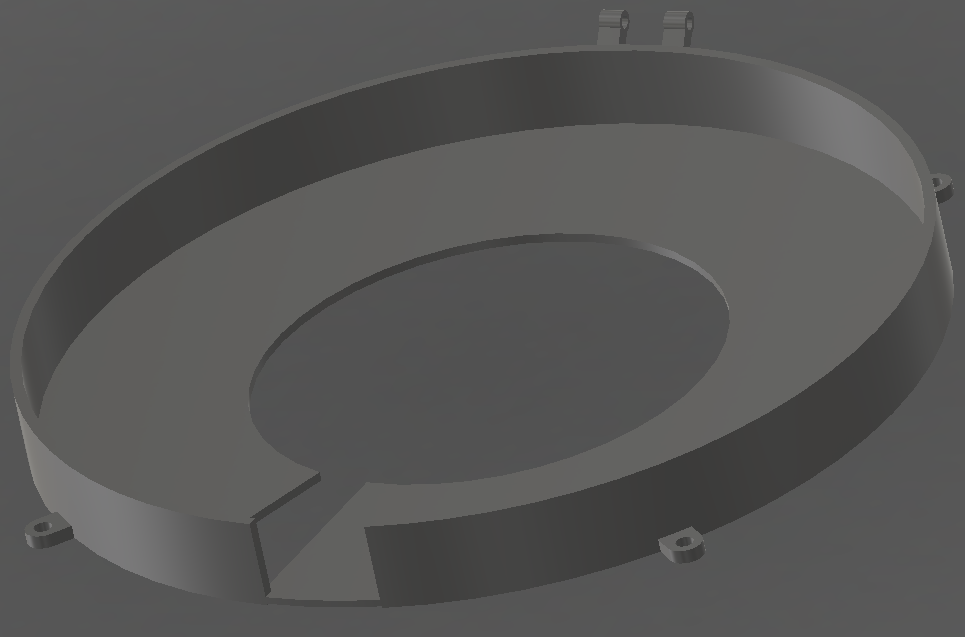
\includegraphics[width=0.7\linewidth]{Figures/Screenshot_6}
	\caption[Upper Body]{Upper Body}
	\label{fig:screenshot6}
\end{figure}
Upper body is a simple design consisting of a cylindrical shape with multiple cutouts. First one is on the floor, through this hole the pills that have not been taken would fall. The other cutout is in the wall, through this cutout the pills that will have to be taken would fall. In the middle there is a circular hole for housing the mill. under the cutout for the dispense pathway, there is a notch to prevent accidental rotation

The measurements are:
\begin{itemize}
	\item outer radius = 100mm
	\item inner radius = 52 mm
	\item height = 20 mm
	\item thickness of floor = 2 mm
	\item thickness of wall = 2.5 mm 
	\item notch depth = 0.4 mm
\end{itemize}
\newpage
\subsubsection{UpperMill}
\begin{figure}[h]
	\centering
	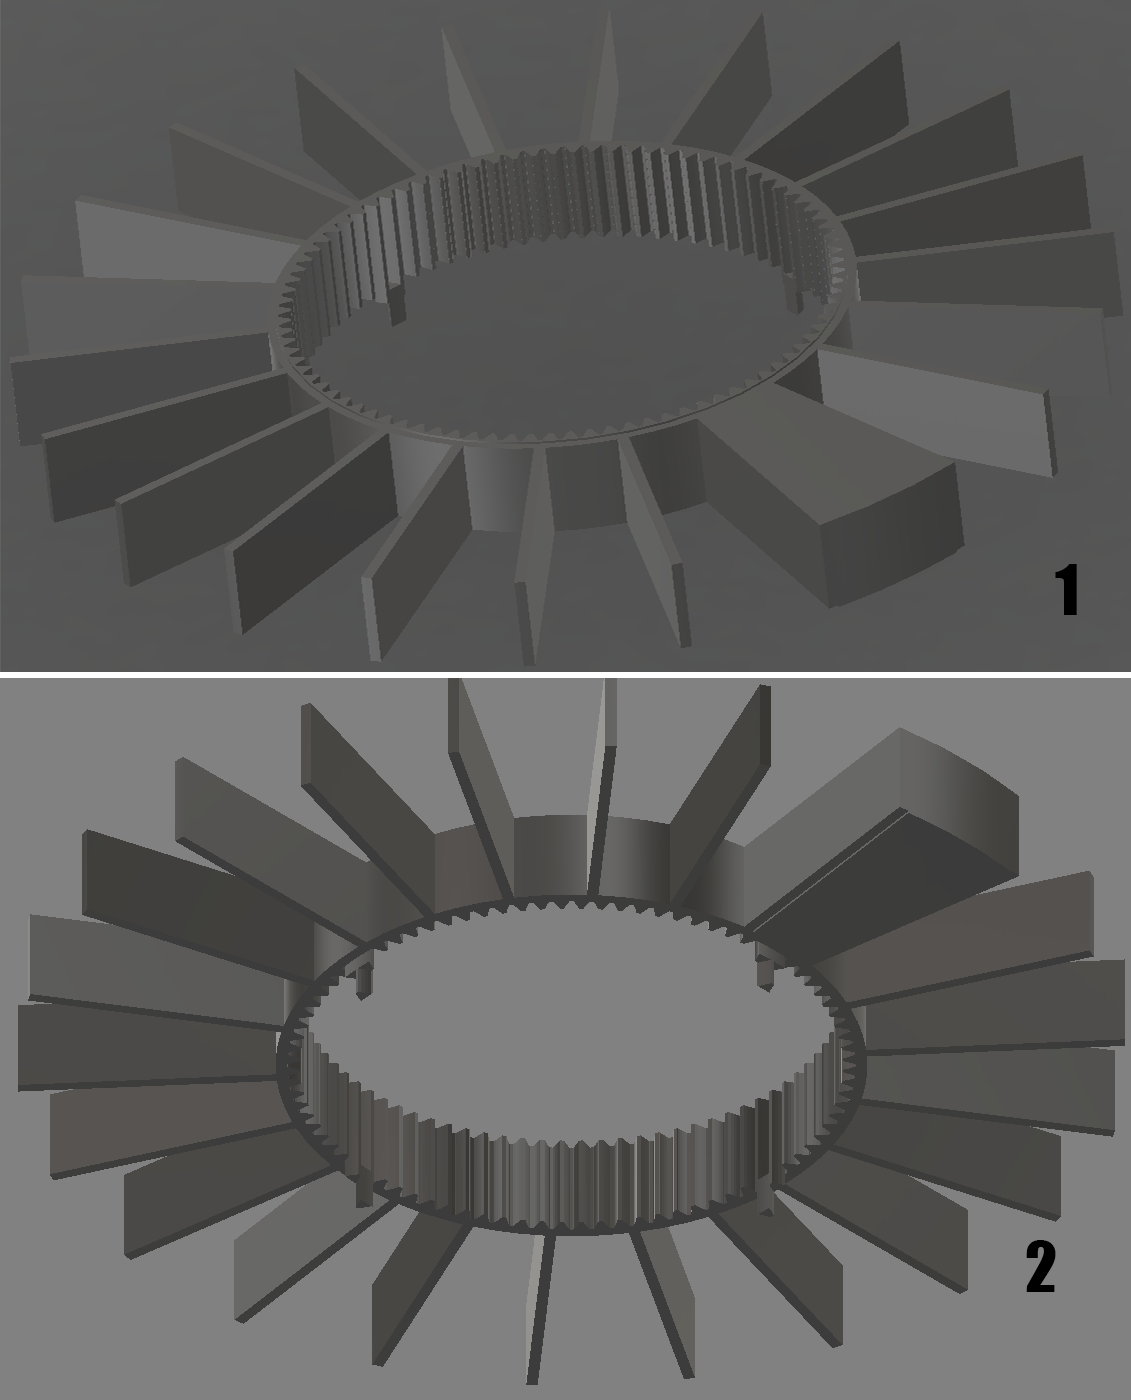
\includegraphics[width=0.6\linewidth]{Figures/Uppermill}
	\caption[Upper Mill]{Upper Mill. 1 View from above. 2 view from below}
	\label{fig:uppermill}
\end{figure}
Upper mill consists of 21 functional chambers and one service chamber. the service chamber is needed to cover the hole in the upper body, so that at any time, 21 chambers are available. Inner rim is designed as a  cogwheel. It has 88 teeth, it will be important later for the stepper motor movement calculation. The gear was designed using a free tool called DXF and SVG GEAR DXF GENERATOR \cite{evolvent_spur_gear_generator}.
These parameters were chosen to match the size of the cog and amount of teeth needed: 
\begin{itemize}
	\item Gear 1 Tooth Count: $-88$ (internal gear)
	\item Gear 2 Tooth Count: $22$
	\item Module: $1.11$ (mm)
	\item Pressure Angle: $20^\circ$
	\item Clearance: $0.15$ mm
	\item Gear 1 Center Hole Diameter: $0$ mm (no hole)
	\item Gear 2 Center Hole Diameter: $0$ mm (no hole)
\end{itemize}

The lower side contains 4 teeth to connect the upper mill to the lower mill. This implementation makes sure that the two mills will move at the same time, removing need for a separate stepper motor for each of them or a connection directly to the upper mill.

There are certain design decisions that have been taken to reduce friction. Firstly, on the upper side the ring is offset by 0.4 mm so that the upper deck will not touch the whole mechanism, but only this ring. At the bottom side, the teeth are complex shaped. the upper part of the tooth has a length of 2.4 mm, which is 0.4 mm taller than the thickness of the floor of the upper body. The idea behind it is that the wings of the mill will not touch the floor directly, leaving 0.2 mm opening between the floor and the upper mill.
 
The measurements of the upper mill are:
\begin{itemize}
	\item chamber height = 17 mm
	\item chamber length = 45.05 mm
	\item inner ring diameter = 100 mm
	\item outer ring diameter = 193 mm
	\item gear tooth depth 2.7 mm
	\item connecting tooth length = 2.4 mm + 5 mm
\end{itemize}
\newpage
\subsubsection{LowerMill}
\begin{figure}[h]
	\centering
	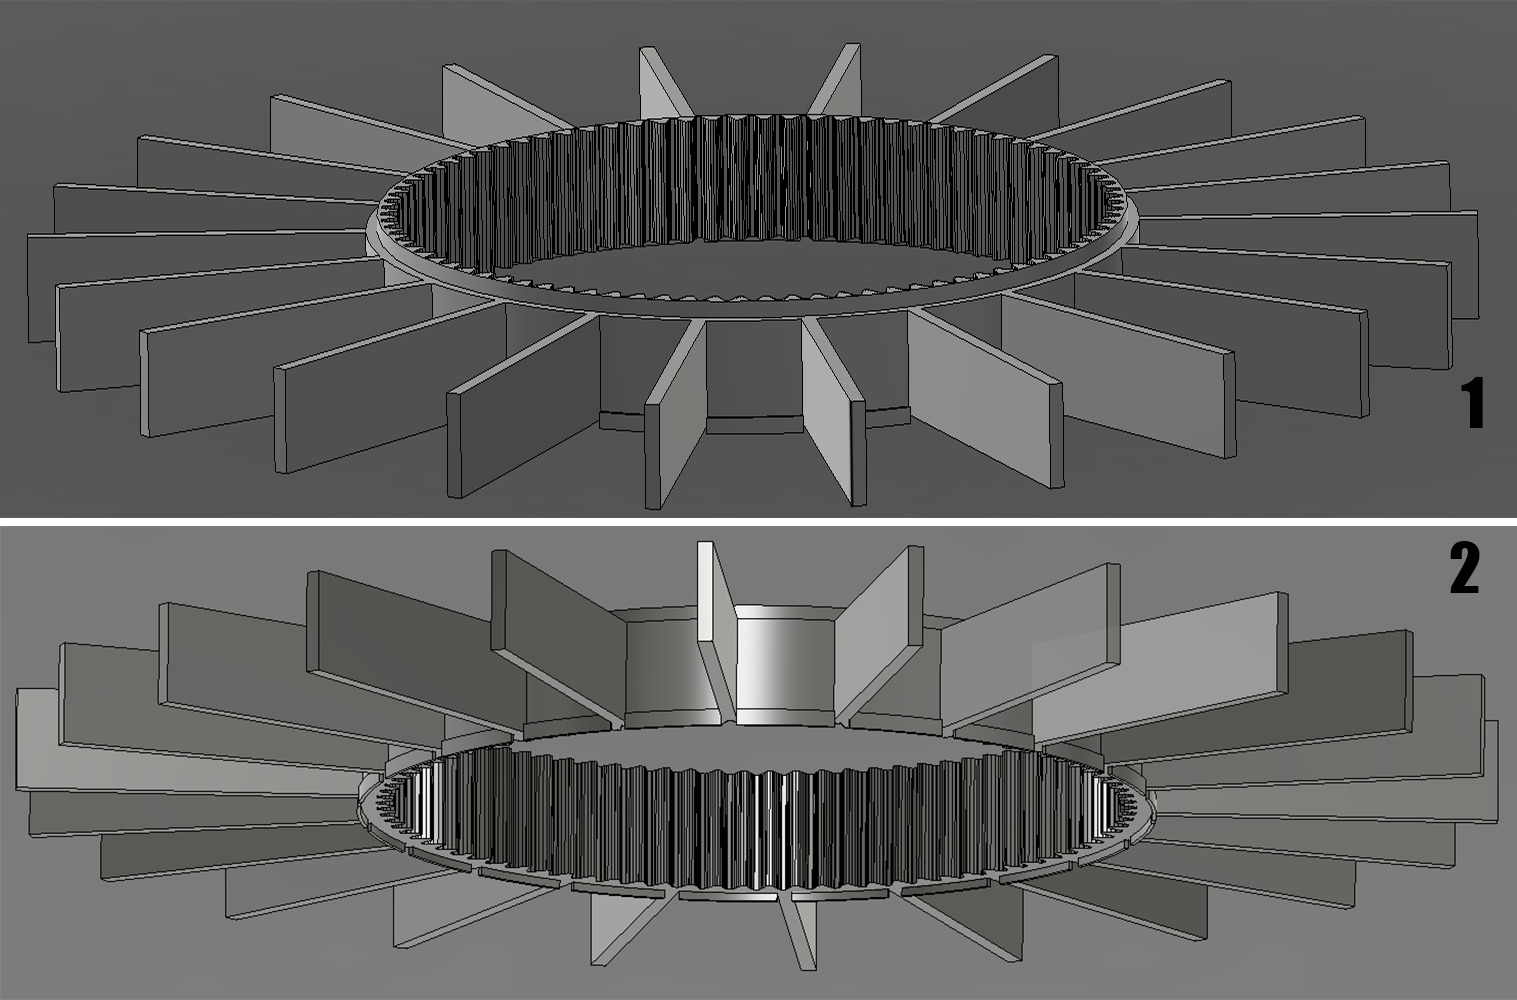
\includegraphics[width=0.7\linewidth]{Figures/Lowermill}
	\caption[Lower Mill]{Lower mill. 1 view from above. 2 view from below}
	\label{fig:lowermill}
\end{figure}
Lower mill consists of 22 chambers which are the same. This is done to make sure that the sizes of upper and lower mill chambers are the same. Just as with the upper mill, inner ring is also a cogwheel, designed the same way and with the same parameters as upper mill. Unlike the upper mill, lower mill doesn't have teeth to connect. The teeth of upper mill are inserted into teeth of cogwheel of the lower mill.

The upper part also contains a ring that is 2 mm above the rest of the construction. This ring exists to eliminate the friction between the ceiling (which is a floor of the upper mill) and the chambers. 

The lower part is also made in such a way as to reduce friction. it contains rims that would travel rotationally along the ring located on the lower body. they are rather tall, measured at 1 mm to make sure that they don't accidentally fall out during movement.

The measurements of lower mill are:
\begin{itemize}
	\item chamber height = 13.6 mm
	\item chamber length = 45.05 mm
	\item inner ring diameter = 100 mm
	\item outer ring diameter = 193 mm
	\item gear tooth depth 2.7 mm
\end{itemize}
\newpage
\subsubsection{LowerBody}
\begin{figure}[h]
	\centering
	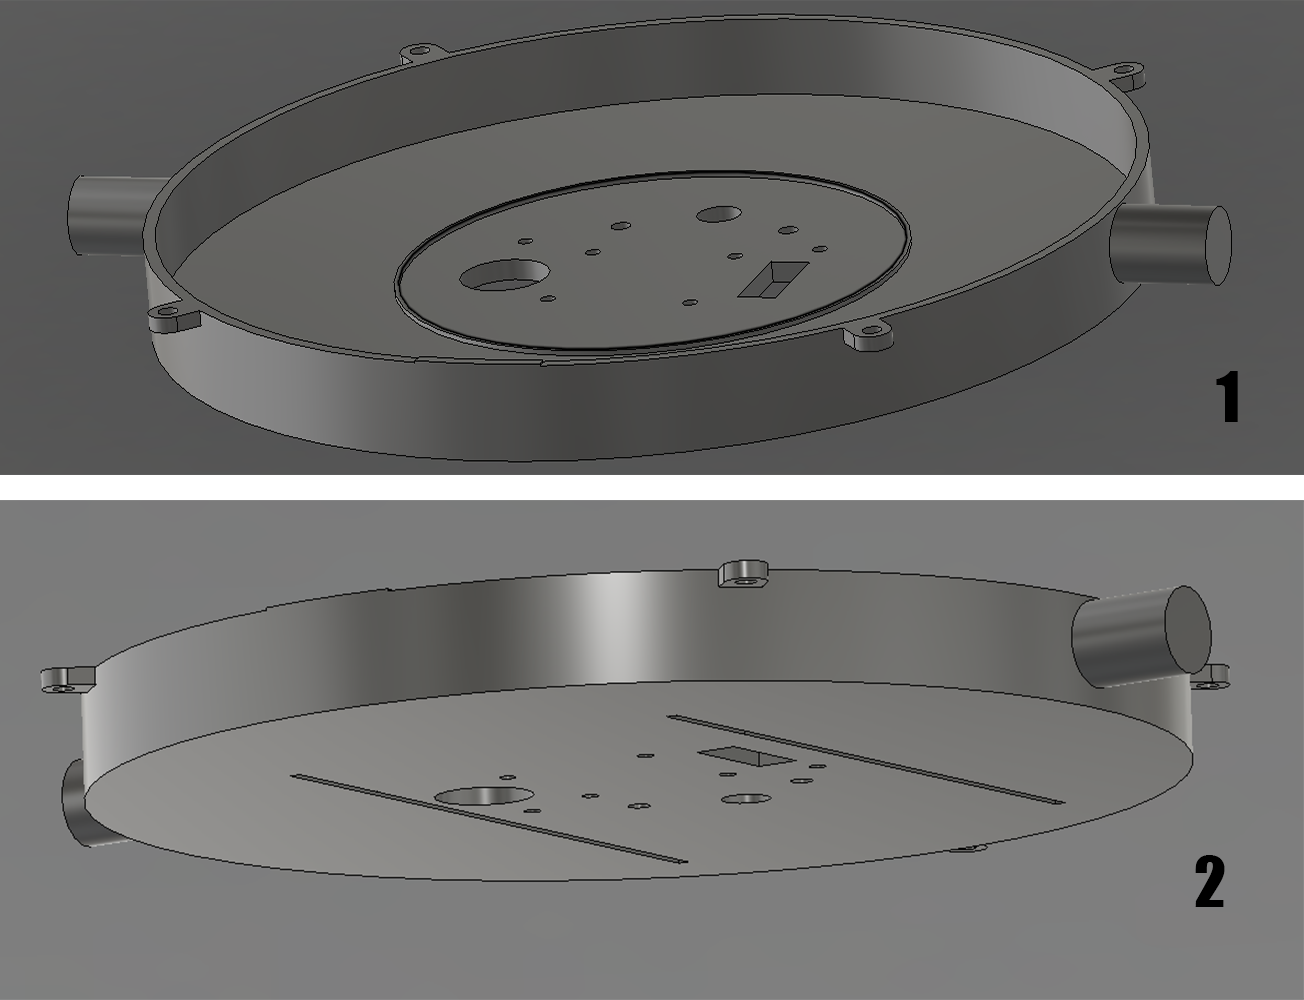
\includegraphics[width=0.7\linewidth]{Figures/Lowerbody}
	\caption[Lower Body]{Lower Body. 1 view from above. 2 view from below}
	\label{fig:lowerbody}
\end{figure}
Lower body is a bit more complex than the upper one. It is designed to connect multiple electronic components, Stepper motor, motor driver - directly, charger and microcontroller - indirectly, through the lower deck.

On the inner side there is a ring around which the lower mill rotates. This ring also separates the chamber area and electronics area. inside this ring there are cutouts for stepper motor, driver and wires.

On the outer side, there are "ears" upon which the whole device would be positioned on a stand. These ears define the axis of rotation for the dispense pathway. Outer rim contains a ridge to fix the the upper body and prevent accidental rotation.

On the inner side there is also grooves to append lower deck, these grooves are needed to remove the possibility of attaching the lower deck the wrong way. Grooves are 125 mm long, 2 mm wide and 2 mm deep.

The measurements of lower body are:
\begin{itemize}
	\item radius = 100mm
	\item ring inner radius = 50.5 mm
	\item ring inner radius = 51.4 mm
	\item ring height = 1 mm
	\item body height = 20 mm
	\item thickness of floor = 4 mm
	\item thickness of wall = 2.5 mm 
	\item notch depth = 0.4 mm
\end{itemize}
\newpage
\subsubsection{Electronics}
\begin{figure}
	\centering
	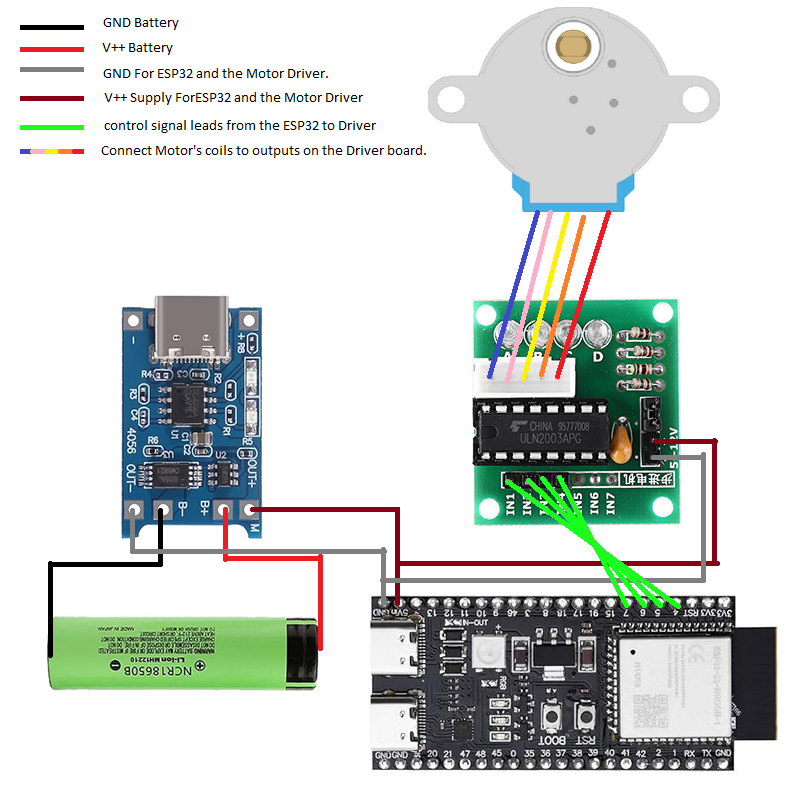
\includegraphics[width=0.5\linewidth]{Figures/Motor}
	\caption[Connection schema of electronic components]{Connection schema of electronic components. Components from top to bottom: 1)28BYJ Stepper motor 2) Left: Charger Module 3)Right: ULN2003 Motor Driver 4)Left:Panasonic NCR18650B Battery 5)Right ESP32 S3 DevKitC-1 N16R8 S3 Microcontroller}
	\label{fig:motor}
\end{figure}
The device needs a microcontroller and a stepper motor for control. There are many options from which to choose, therefore we need to know what we need for our electronics to filter out possible choices. Microcontroller needs to be able to control a stepper motor and also to have a network interface, Wi-Fi or Bluetooth, so that we can host an user interface somewhere else. Stepper motor needs to have enough torque to rotate 2 mills and a load. We don't need a high performance stepper motor, since our rotational speed is not that important. also it should be noticed that there is a gear reduction of 4:1 on the gears which results in 4 times higher torque for 4 times lower speed. From the measurements above we know that the diameter of mill is 200 mm, the weight is hard to calculate, but we can access the calculation used by the slicer software. The results are 44 g for Lower mill, and 61 g for Upper mill for 105g in total. The extra weight from pills would be around 100g for 205g in total. While there has been no calculation involved, the setup was tested with the coins to serve as a load, however it was tested only with the lower mill attached. We will come back to discuss the results in the later part of the document. Considering also that the one of the goals of the project was to develop the device for as cheap as possible, a 28BYJ \cite{stepper} stepper motor was chosen, together with the ULN2003\cite{ti_uln2003a_revT_2025} Motor driver.

For the microcontroller, an ESP32 S3 DevKitC-1 N16R8 ESP32 S3 was selected \cite{microcontroller}. it is a common choice to pair this microcontroller and stepper motor and it has the network interface (both Wi-Fi and Bluetooth). For us a Bluetooth-Low-Energy is of particular interest. It allows us to save battery, since we don't need a constant stream of data exchange between a smartphone and device.

Another addition to the electronics is inclusion of battery. While not a requirement, battery-powered device is much more convenient to use as it makes it independent from being located near a socket. For this, Panasonic NCR18650B \cite{panasonic_ncr18650b} Battery was selected. 
\newpage
\subsubsection{Lower Deck(Electronics compartment)}
\begin{figure}[h]
	\centering
	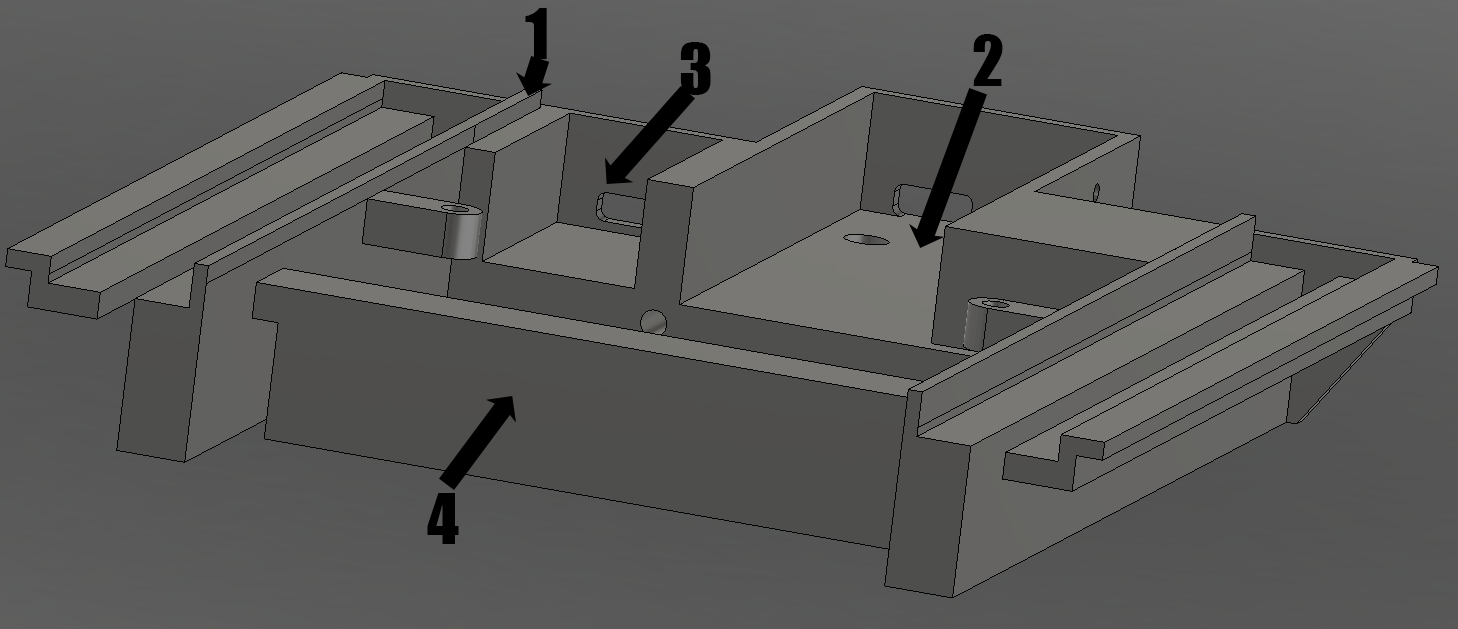
\includegraphics[width=0.7\linewidth]{Figures/Screenshot_13}
	\caption[Lower Deck]{Lower Deck and its' features: 1)Ridge 2)Microcontroller housing 3)Charger Module housing 4)Battery Wall}
	\label{fig:screenshot13}
\end{figure}
The lower deck houses three electronic components: Microcontroller, battery charger and battery. It also serves as a cover for the stepper motor, whereas the driver would be located on the opposite side of the lower body, inside the ring. The shape of the lower deck is quite more complex than that of the previous bodies, therefore it makes sense to divide the description of it into multiple parts. on the image \ref{fig:screenshot13} you can see the lower deck and a numbers that point to the parts of components. Here is a description of all the components of this body:
\begin{enumerate}
	\item{\textbf{Ridge}} Lower body has 2 parallel grooves on its lower part. These grooves will house these ridges on the lower deck. The ridges are designed to actually be a tiny bit smaller (1.6 mm vs 2 mm) than the notches of the lower body, we will discuss why in the later chapter. Ridges are 125mm long, 1.6 mm thick and 2 mm deep. 
	\item{\textbf{ISP32 Microcontroller housing}} This is where the microcontroller would be placed. We know the dimensions of the microcontroller (63.5 mm x 28 mm) and this opening is made to be around the same size to fit it (67.6 mm x 28 mm). It has cutouts on the body for 2 USB ports present on a microcontroller, as well as a LED.
	\item{\textbf{Charger Module housing}} In this part the charger circuit will be nested. The cutout matches exactly the dimensions of the charging module (28 mm x 17.5 mm). This compartment contains also the cutout on the body for the USB port.
	\item{\textbf{Battery Wall}} Battery holder is attached to this wall. at the sides one can notice that the connection to the side walls does not go all the way. The reason is that wires will go from the battery holder through these openings. 
\end{enumerate}
Lower deck also features a long hole for a slide-in lid which you can see to the sides from the Ridges that connect Deck to the lower body.
\newpage
\subsubsection{Stand}
\begin{figure}[h]
	\centering
	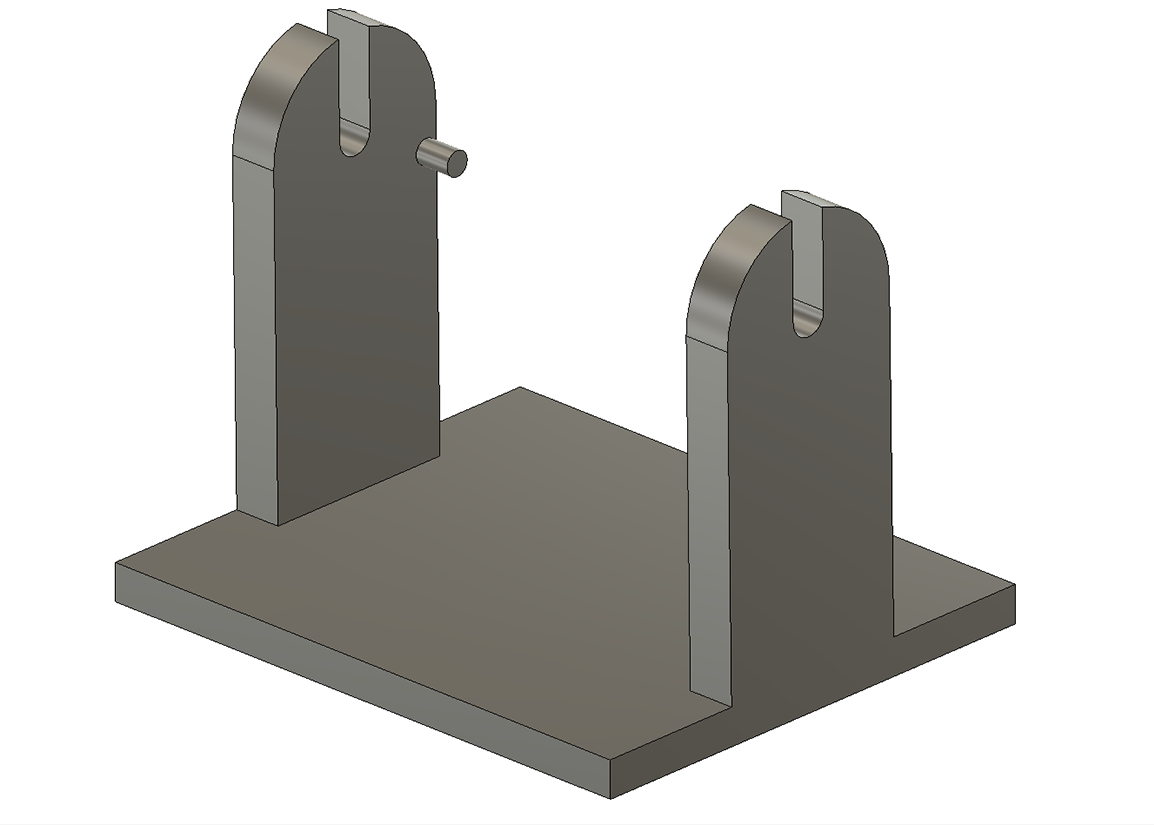
\includegraphics[width=0.7\linewidth]{Figures/Screenshot_14}
	\caption[Stand]{Stand}
	\label{fig:screenshot14}
\end{figure}
Stand is a simple design that features 2 distinct components: Pillars to the sides to hold the device and a dispensing dock in the front and center of it. The pillars have a cutout to slide down the device into it and notches to prevent the device from tilting backwards. The dispensing dock is designed to match the shape of the device so that it can easily be tilted into it at a 45 degree angle.
The dimensions are:
\begin{itemize}
	\item Stand height from bottom to the peak of stand: 190 mm
	\item Stand Width: 240 mm
	\item Stand Length: 200 mm
	\item Stand floor thickness: 15 mm
	\item Pillar thickness: 20 mm
\end{itemize}

It should be noted, however, that although this Stand is the default solution for the sake of completeness of the project, ideally, it would be manufactured not with a plastic, but rather with metal. The purpose of the stand (besides providing pathway for dispense of the pills) is also to provide stability of the construction so that people suffering from tremors would be able to lean firmly onto it and stabilize their hand. In this case, plastic might not be the optimal solution.
\newpage
\subsection{3D printing specifics}
As mentioned earlier, one of the goals of the project is to make the device buildable with consumer-grade devices, among them 3D-Printers. This requirement introduces first physical limitations for the device, as 3D-Printers have a limited printing space. For this project as a reference printer, a Prusa MK4S 3D-Printer \cite{PrusaMK4Specs} was selected. From the Specification we can see that the build volume is 250 x 210 x 220 mm, putting a limitation on how large our device can be. Theoretically, of course, we could circumvent this limitation by designing the components in such a way that they would consist of multiple parts interlocking with themselves, however this adds unnecessary complexity to an already extensive project. The dimensions of each component mentioned in previous section conform to this limitation.

As for material selection, Prusa MK4S (and many other printers) support printing with PLA plastic. This material has many advantages: it is biodegradable (it is a polymer of lactic acid), lightweight, sterile, doesn't produce as much fumes as standard ABS plastic and is easy to print with. However, certain disadvantages should be mentioned: Heat deflection at around 55-60 degrees means it cannot be washed with boiling water as it would warp the body. Pure PLA is food safe, however the pigments might not be, so any wear might introduce microparticles that might not be as safe to consume if colored PLA is chosen.
